Precision measurement of the gauge boson couplings is a well known
method to look for physics beyond the Standard Model. In the case of
the triple gauge boson couplings, new physics contributions can be
expressed in the form of an effective Lagrangian. The most general
form of such a Lagrangian has 14 complex couplings (7 for $WWZ$ and 7 for
$WW\gamma$). Assuming electromagnetic gauge invariance, and C and P
symmetry conservation that number is reduced to five:
$\Delta\kappa_Z$, $\Delta g^Z_1$, $\Delta\kappa_{\gamma}$, $\lambda_Z$
and $\lambda_{\gamma}$. Applying gauge constraints:
\begin{align}
  \Delta\kappa_Z &= \Delta g^Z_1- \Delta\kappa_{\gamma}\tan^2\theta_W \\
  \lambda_Z &= \lambda_{\gamma}
\end{align}
further reduces the number of independent couplings to three. In the
Standard Model all five couplings are zero. 
 
CMS performed a first measurement of the anomalous couplings with
35/pb of data at 7 TeV~\cite{Chatrchyan:2011tz}. The measurement was performed with
and without a form factor that helps to avoid unitarity violation by
introducing an effective cutoff scale where a coupling is switched
off.  In this study we have two orders of magnitude more data and
experimental constraints on the couplings are more stringent then the
unitarity constraint. Therefore all the anomalous couplings are
form-factor free.

This analysis is based on the $W^+W^-$ production cross-section
measurement in $\intlumi$ of $pp$ collision data at $\sqrt{s} = $
7~$\TeV$ (the full 2011 dataset) \cite{ref:WWXS2011}. 
The main kinematic observable is the leading lepton $p_T$ distribution,
shown after all event selections in Figure \ref{fig:pas_pt1_incl}.

The datasets, event selections and background estimates are the 
same as those used in Reference \cite{ref:WWXS2011}, where
they are described in detail.
Here we re-summarize the datasets and event selections
in brief in Sections \ref{sec:datasets} and \ref{sec:selection}.

\begin{figure}[t]
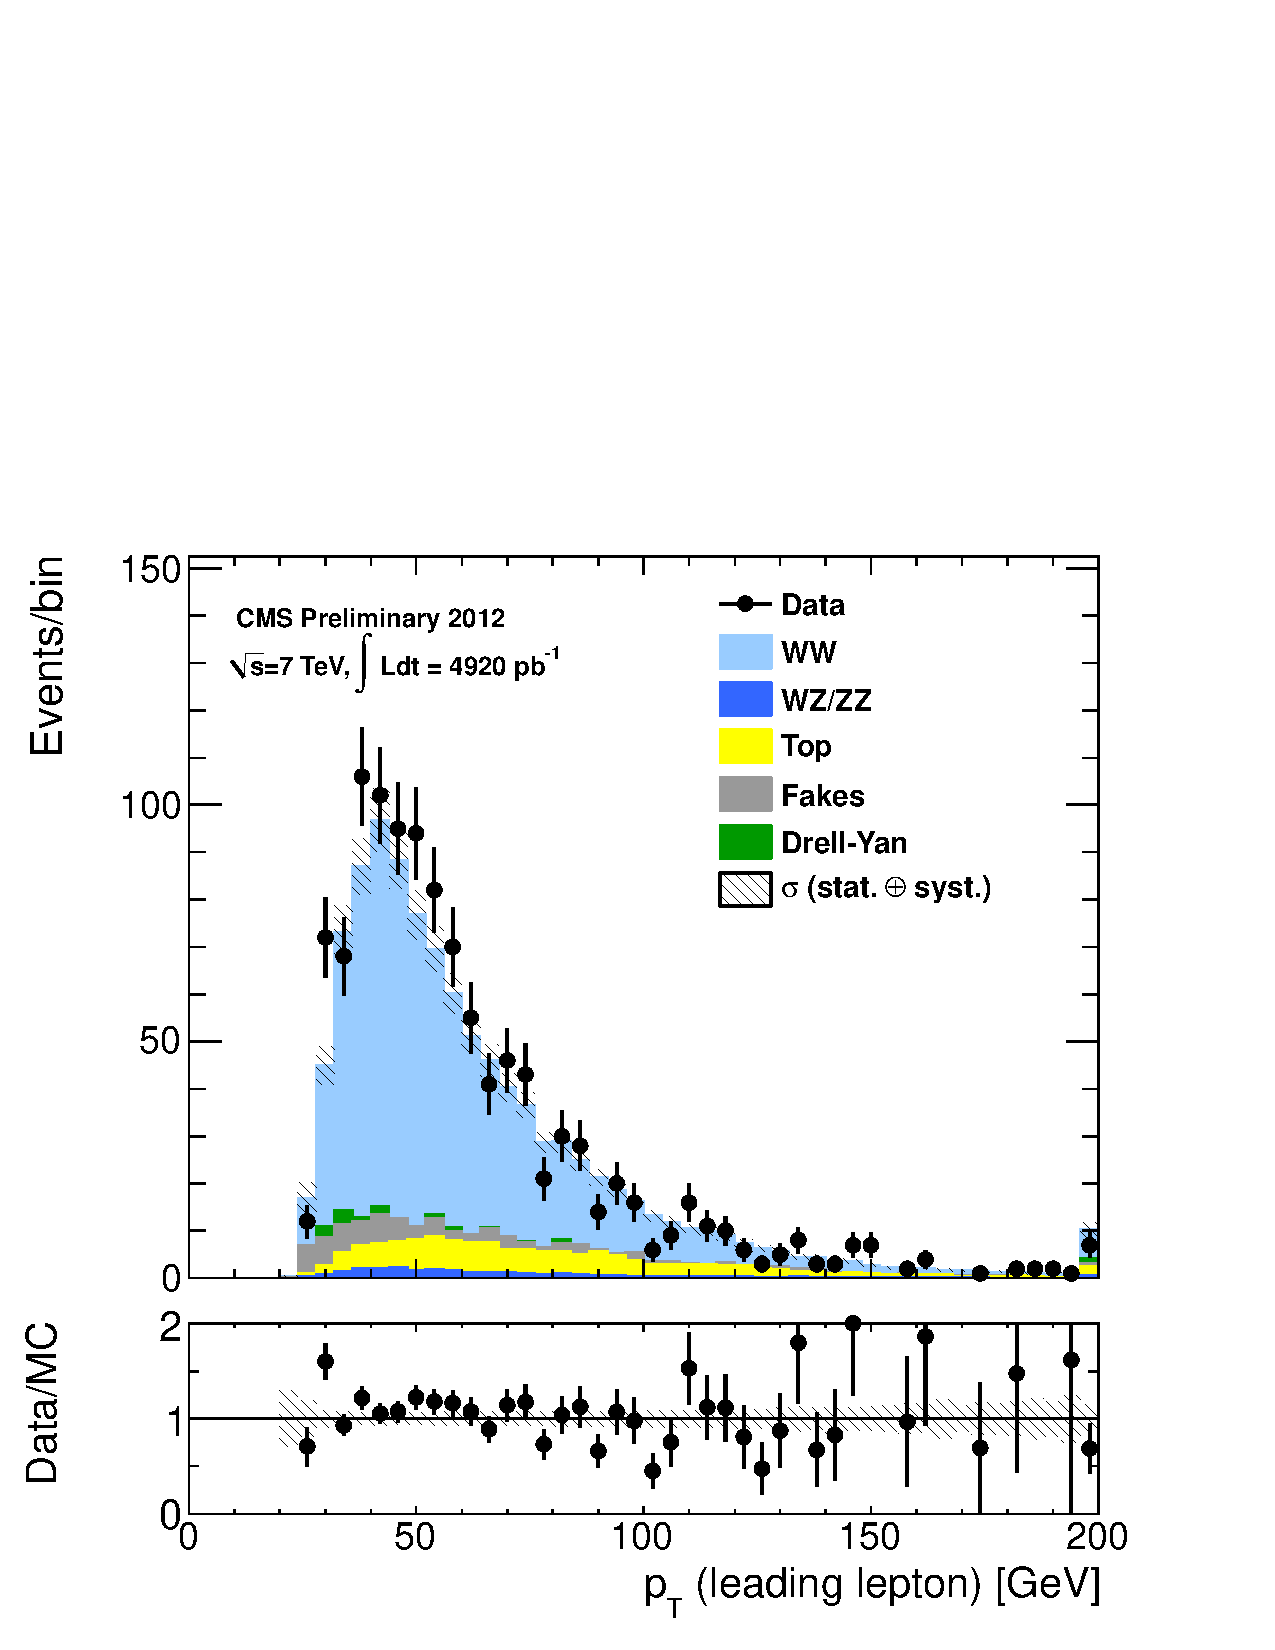
\includegraphics[width=.45\textwidth]{figures/pas_pt1_incl.pdf}
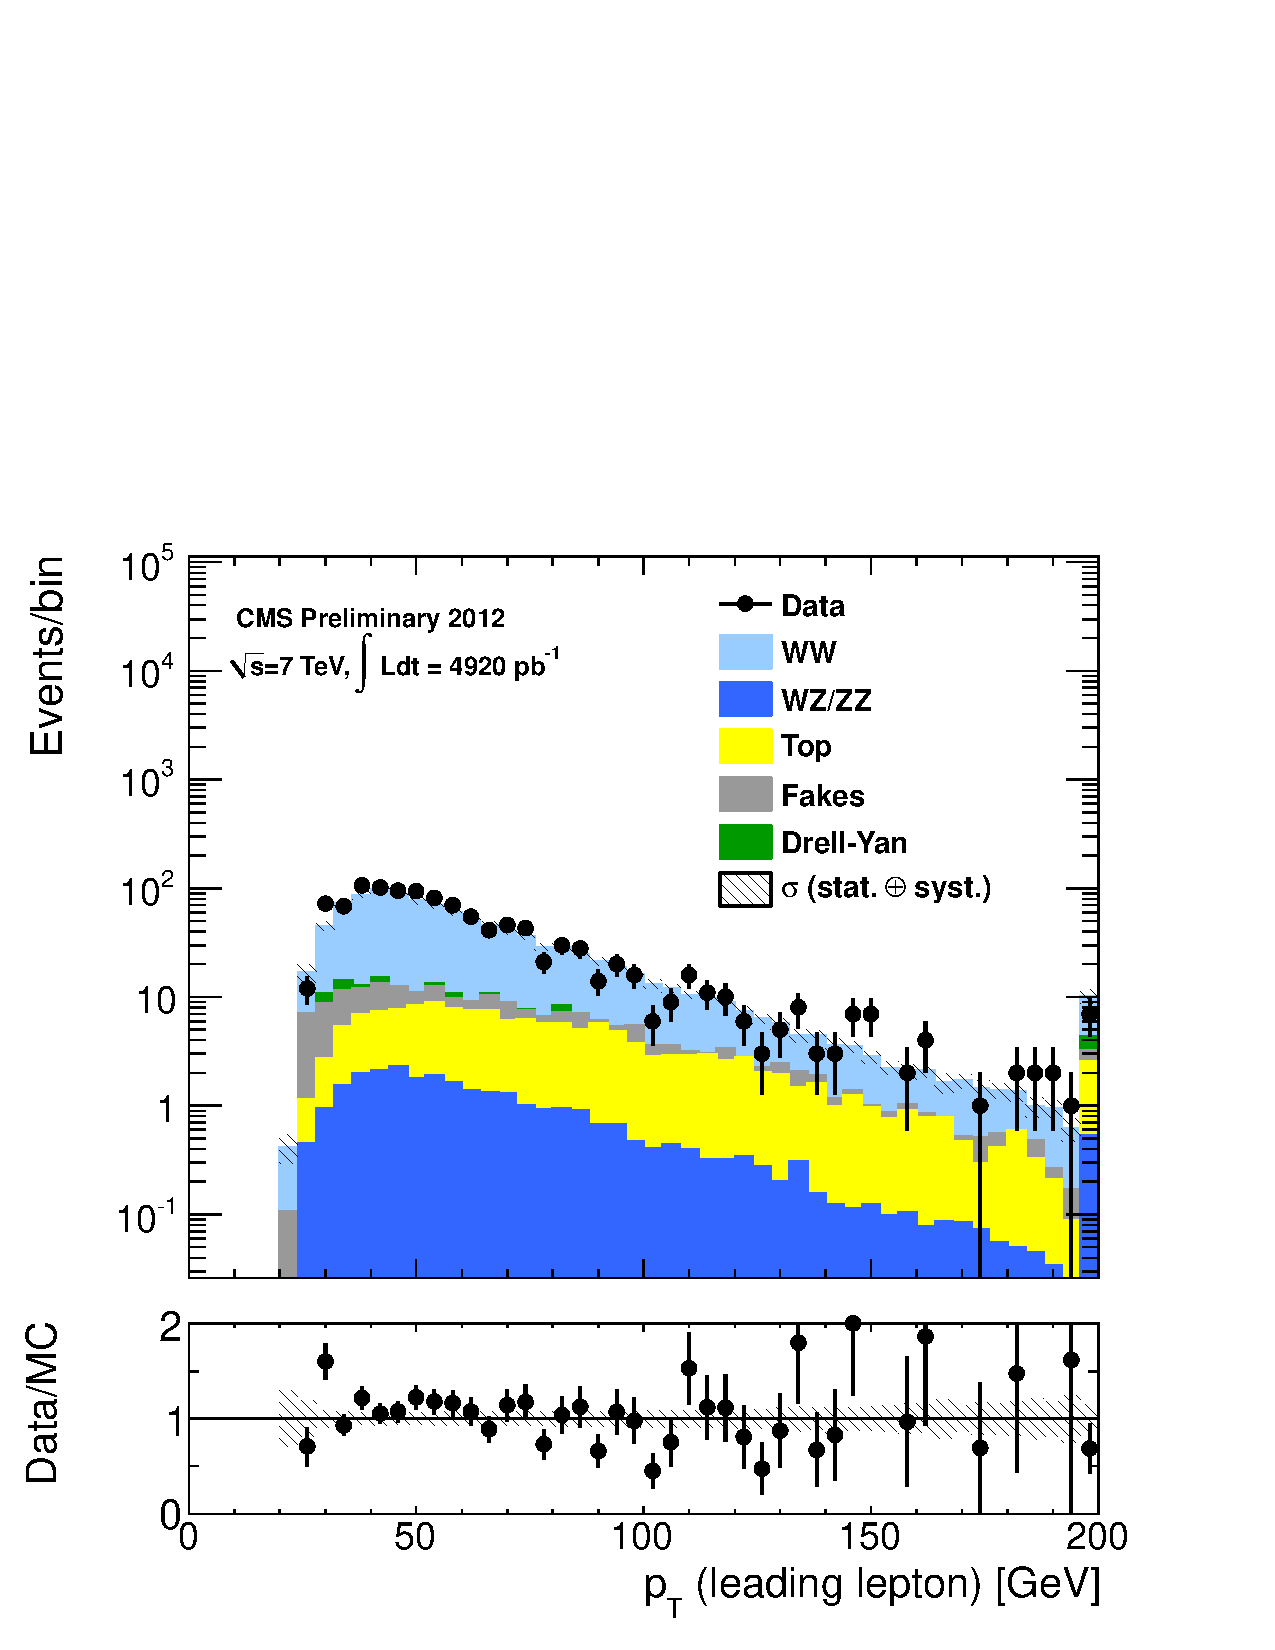
\includegraphics[width=.45\textwidth]{figures/pas_pt1_incl_log.pdf}
\caption{Leading lepton \pt distribution on linear (left) and logarithmic (right) scale.}
\label{fig:pas_pt1_incl}
\end{figure}

